% Tier 1 parity doc: TikZ graphics — heavy primitive/box/whatsit usage.
% Exercises specials, rules, kerns, and deep box nesting via pgf.
\documentclass[11pt]{article}
\usepackage{tikz}
\usetikzlibrary{arrows.meta,positioning}
\begin{document}
\section*{TikZ}

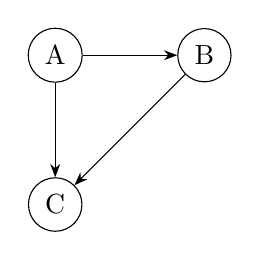
\begin{tikzpicture}[node distance=12mm,>=Stealth]
  \node[draw,circle] (a) {A};
  \node[draw,circle,right=of a] (b) {B};
  \node[draw,circle,below=of a] (c) {C};
  \draw[->] (a) -- (b);
  \draw[->] (a) -- (c);
  \draw[->] (b) -- (c);
\end{tikzpicture}

\bigskip

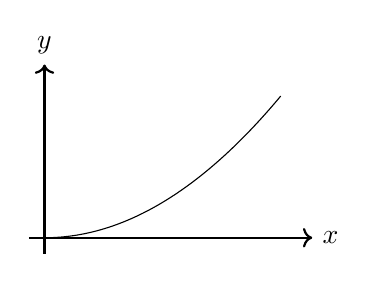
\begin{tikzpicture}
  \draw[thick,->] (-0.2,0) -- (3.4,0) node[right] {$x$};
  \draw[thick,->] (0,-0.2) -- (0,2.2) node[above] {$y$};
  \draw[domain=0:3,smooth,samples=50] plot (\x,{0.2*\x*\x});
\end{tikzpicture}

\end{document}
